\appendix
\Huge{\textbf{Appendices}}

\section{Augmented Images}\label{apx:augmentedImages}

\begin{figure}[h]
    \centering
    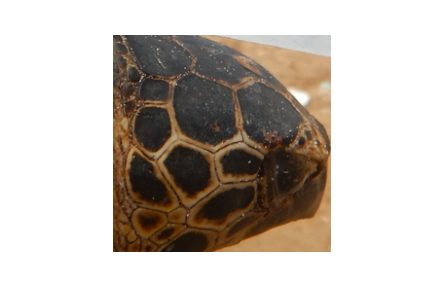
\includegraphics{images/turtles/augmented/base.png}
    \caption{Non-augmented image.}
    \label{fig:turtleBase}
\end{figure}

\begin{figure}
    \centering
    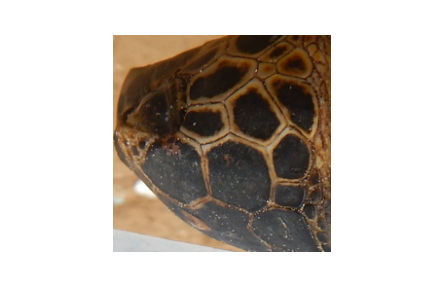
\includegraphics{images/turtles/augmented/rotated.png}
    \caption{Image rotated by 180 degrees.}
    \label{fig:turtleRotated}
\end{figure}

\begin{figure}
    \centering
    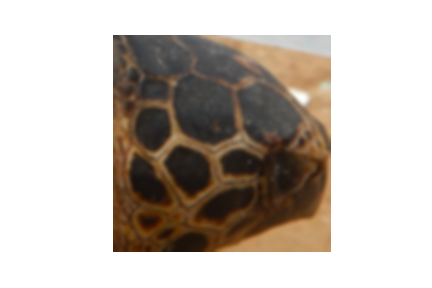
\includegraphics{images/turtles/augmented/gaussian.png}
    \caption{Image with Gauss-filter applied.}
    \label{fig:turtleGauss}
\end{figure}

\begin{figure}
    \centering
    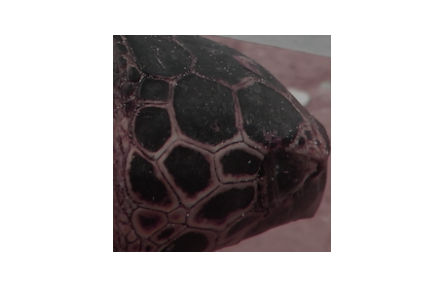
\includegraphics{images/turtles/augmented/hsv.png}
    \caption{Image with randomly changed HSV values.}
    \label{fig:turtleHSV}
\end{figure}

\begin{figure}
    \centering
    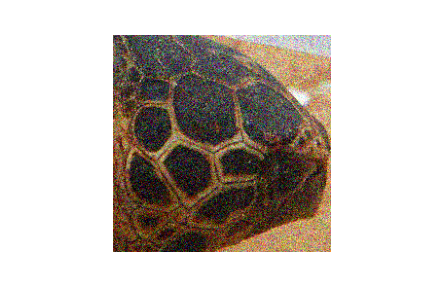
\includegraphics{images/turtles/augmented/noise.png}
    \caption{Image with added noise.}
    \label{fig:turtleNoise}
\end{figure}